\documentclass[9pt]{IEEEtran}

\usepackage[english]{babel}
\usepackage{graphicx}
\usepackage{epstopdf}
\usepackage{fancyhdr}
\usepackage{amsmath}
\usepackage{amsthm}
\usepackage{amssymb}
\usepackage{url}
\usepackage{array}
\usepackage{textcomp}
\usepackage{listings}
\usepackage{hyperref}
\usepackage{xcolor}
\usepackage{colortbl}
\usepackage{float}
\usepackage{gensymb}
\usepackage{longtable}
\usepackage{supertabular}
\usepackage{multicol}

\usepackage[utf8x]{inputenc}

\usepackage[T1]{fontenc}
\usepackage{lmodern}
\input{glyphtounicode}
\pdfgentounicode=1

\graphicspath{{./figures/}}
\DeclareGraphicsExtensions{.pdf,.png,.jpg,.eps}

% correct bad hyphenation here
\hyphenation{op-tical net-works semi-conduc-tor trig-gs}

% ============================================================================================

\title{\vspace{0ex}Long-Term Tracking}

\author{Marko Rozman\vspace{-4.0ex}}

% ============================================================================================

\begin{document}

\maketitle

\section{Introduction}

I this report I describe my work on the long-term tracking assignment. The goal of the assignment is to implement a long-term tracker that can recover from occlusions and other problems that cause the tracker to lose the target. 


\section{Task 1}
My PC does not have a GPU, so I'll be working on fewer number of sequences. I downloaded the required files and ran the SiamFC tracker on the sequence car9. The tracker was able to track the car until it passed under the sign. Then the tracker lost the car and was unable to recover. I got the following results \ref{tab:results_1}

\begin{table}[H]
    \centering
    \begin{tabular}{|c|c|c|c|}
    \hline
    Precision & Recall & F-score \\
    \hline
    0.63 & 0.27 & 0.38 \\
    \hline
    \end{tabular}
    \vspace{0.5em}
    \caption{Tracker performance}
    \label{tab:results_1}
    \end{table}



\section{Task 2}
I split the update function into two functions one to detect and one to update. The update function decides if it should work as a tracker or if the object is lost and it should switch to search. The search mode searches in random points on the image, using a bounding box the same size as last tracked frame. This makes the assumption that the tracked object will not change size while it's hidden. This is not a good assumption. While the tracker is searching it's returning the last known position. To set the treshold I looked at the max responses of the tracker on the car9 sequence and decided to set the start search treshold at 4 and the treshold for successful detection at 4,5.  The tracker was able to redetect the car after it passed under the sign and continiued to track it till the end. \ref{tab:results_2}
\begin{table}[H]
    \centering
    \begin{tabular}{|c|c|c|c|}
    \hline
    Precision & Recall & F-score \\
    \hline
    0.60 & 0.59 & 0.59 \\
    \hline
    \end{tabular}
    \vspace{0.5em}
    \caption{Tracker performance}
    \label{tab:results_2}
    \end{table}  

\section{Task 3}
I defined the confidence score as the maximum response of the tracker. To find the best treshold I would run the tracker with diffrent tresholds on the whole dataset and look for best F1 score. Since I don't have a GPU I ran the tracker only on sequnce cat1. The sequence car9 seemed to simple since the car appears back in nearly the same position. \ref{fig:confidence_score}

\begin{figure}
    \centering
    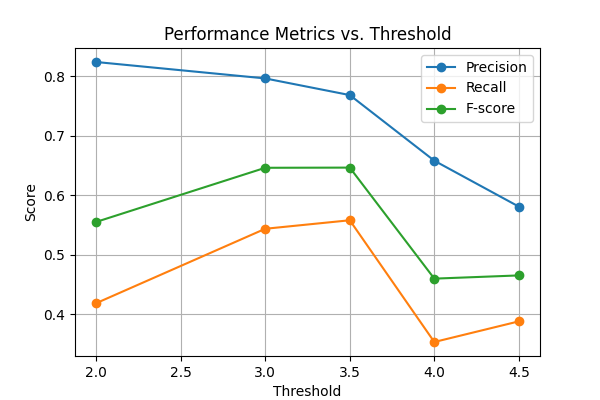
\includegraphics[width=1\columnwidth]{../figs/figure3.png}
    \caption{We can see that the F1 score rises and then falls as the treshold increases. A too low treshold will cause the tracker to start tracking other object that return a response and never trigger the search mode, a too high treshold will cause the tracker to always search and never track.}
    \label{fig:confidence_score}
\end{figure}

\section{Task 4}
Too see the effect of the number of points, we could look at the F1 score while the number of points change. I predict a bigger number of points would cause the tracker to find the target sooner, but would quickly become a performance bottleneck. I tried changing the nuber of points on the sequence cat1 but got inconclusive results. Since the cat is always quite big in the frame, even a small number of points quickly finds it. \ref{fig:incinclusive}

\begin{figure}
    \centering
    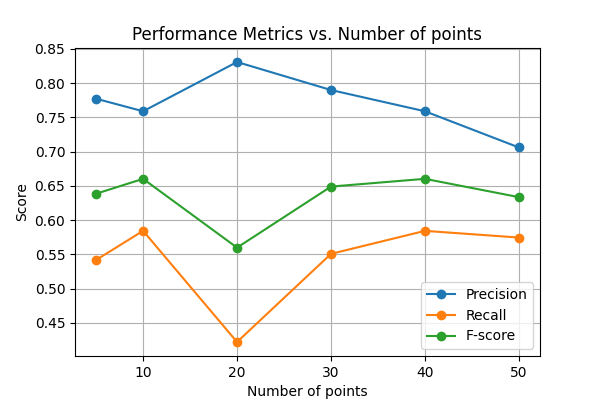
\includegraphics[width=1\columnwidth]{../figs/figure4.png}
    \caption{Inconclusive results on the number of points.}
    \label{fig:incinclusive}
\end{figure}

\section{Task 5}
\begin{figure}[H]
    \centering
    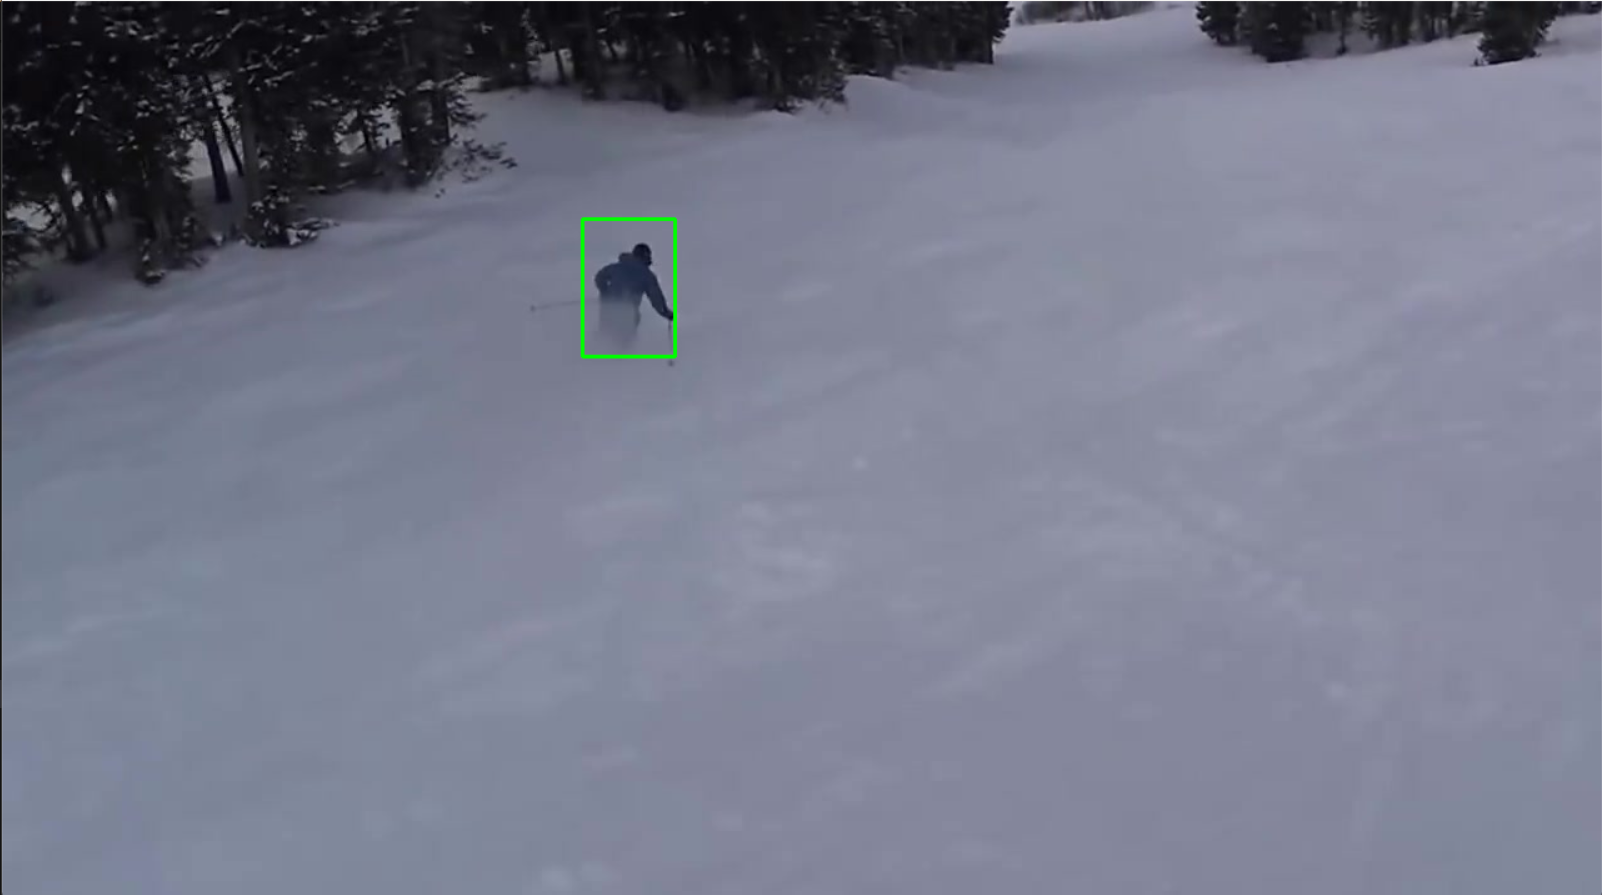
\includegraphics[width=0.48\columnwidth]{../figs/1_frame_50.png} \hfill % Row 1, Image 1
    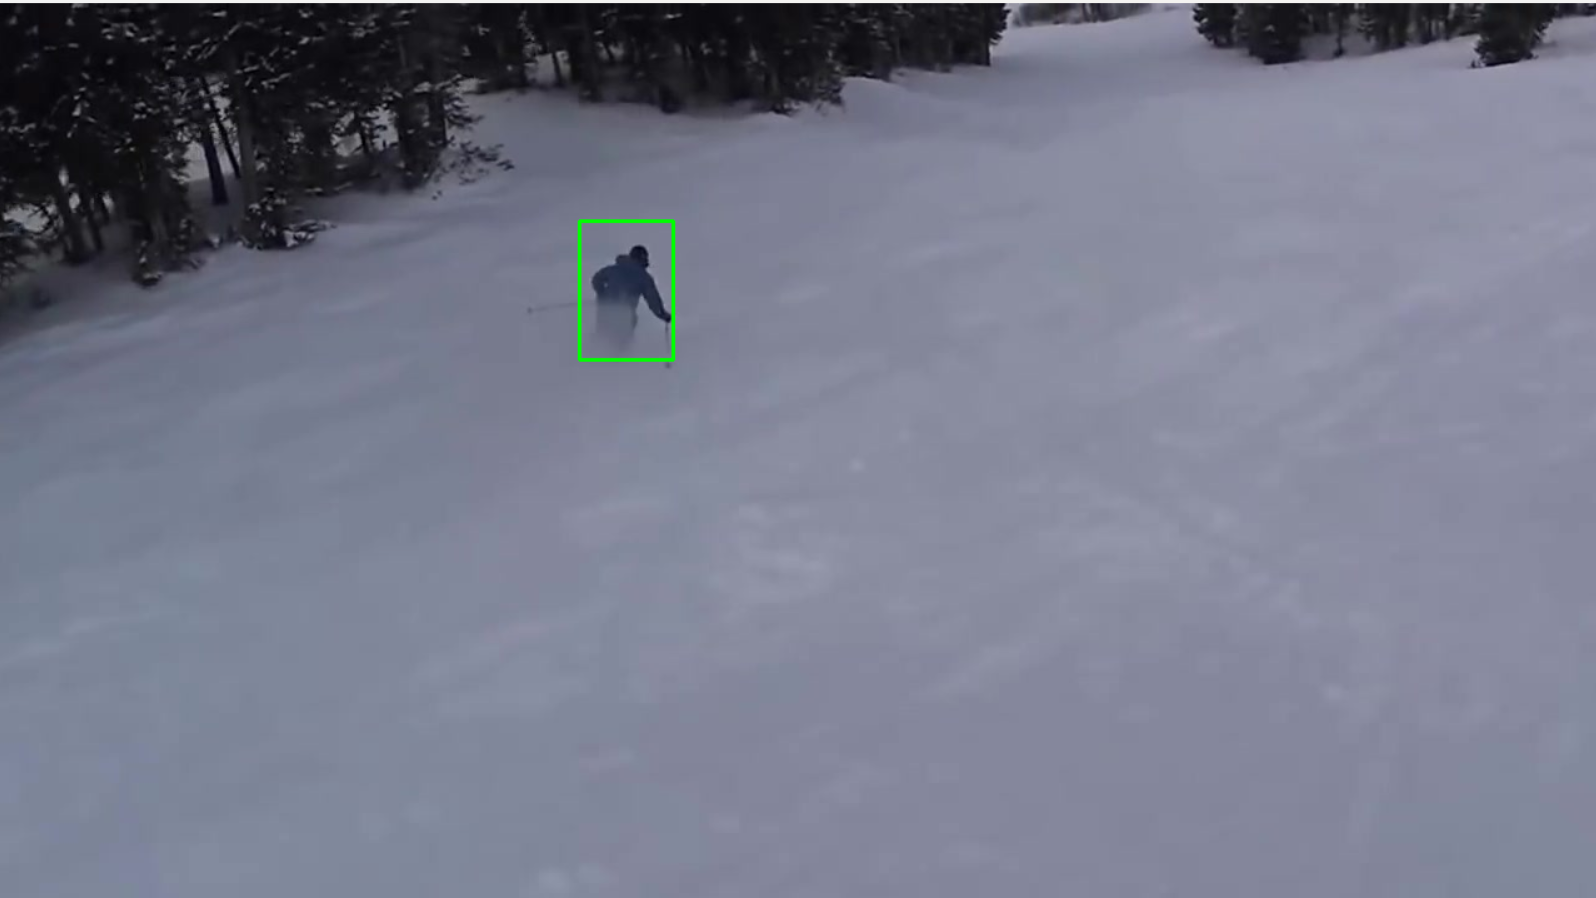
\includegraphics[width=0.48\columnwidth]{../figs/2_frame_50.png} \\ % Row 1, Image 2
    \vspace{1ex} % Vertical space between rows
    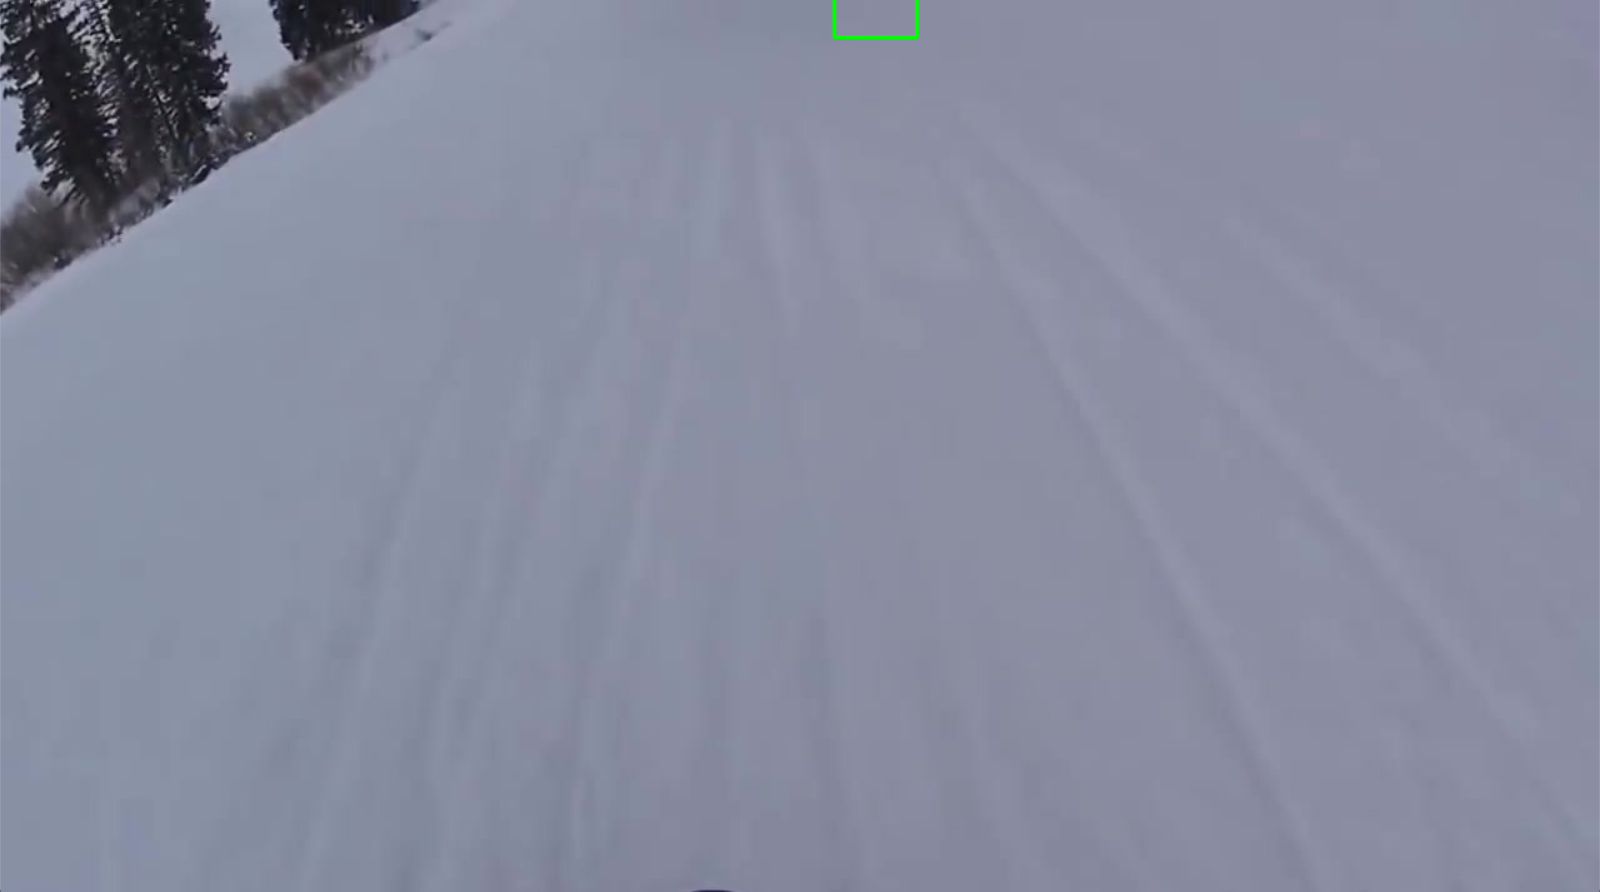
\includegraphics[width=0.48\columnwidth]{../figs/1_frame_271.png} \hfill % Row 2, Image 1
    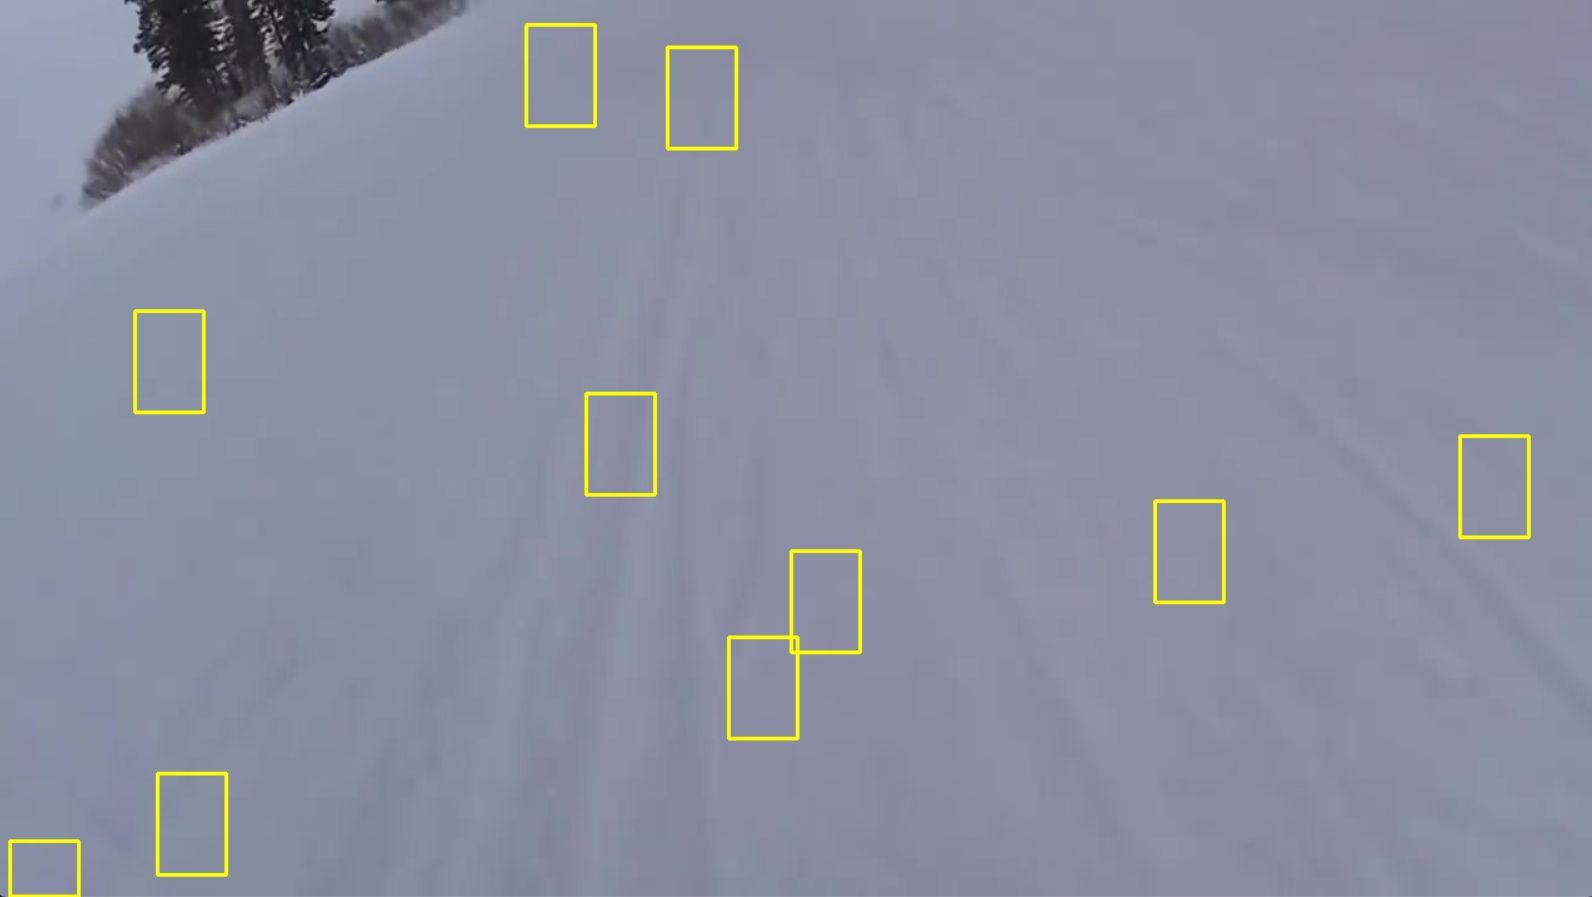
\includegraphics[width=0.48\columnwidth]{../figs/2_frame_260.png} \\ % Row 2, Image 2
    \vspace{1ex} % Vertical space between rows
    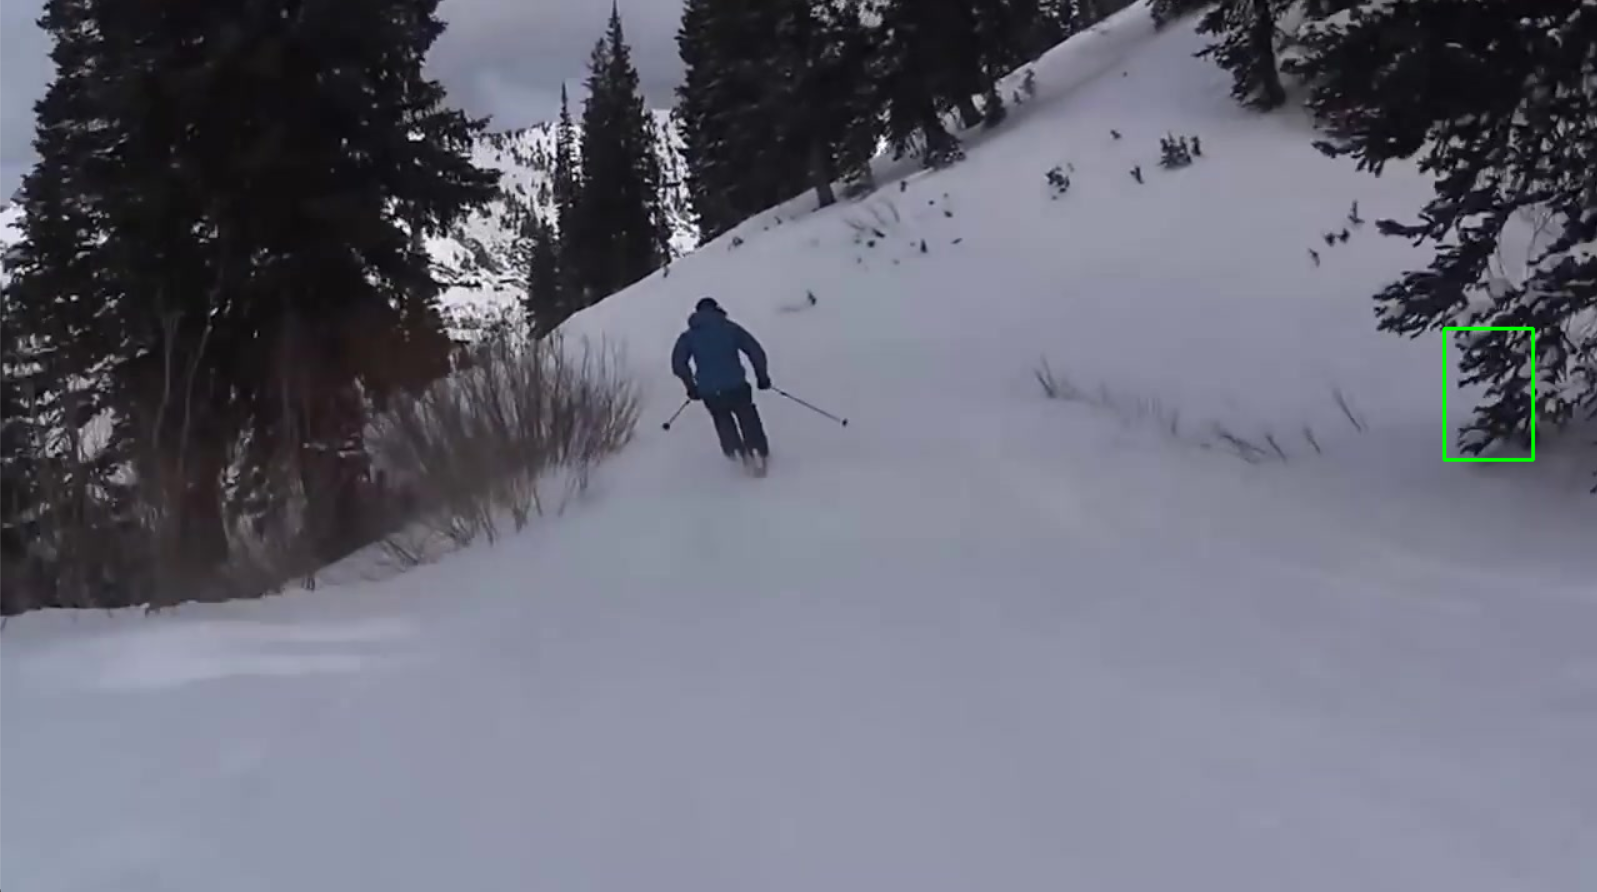
\includegraphics[width=0.48\columnwidth]{../figs/1_frame_372.png} \hfill % Row 3, Image 1
    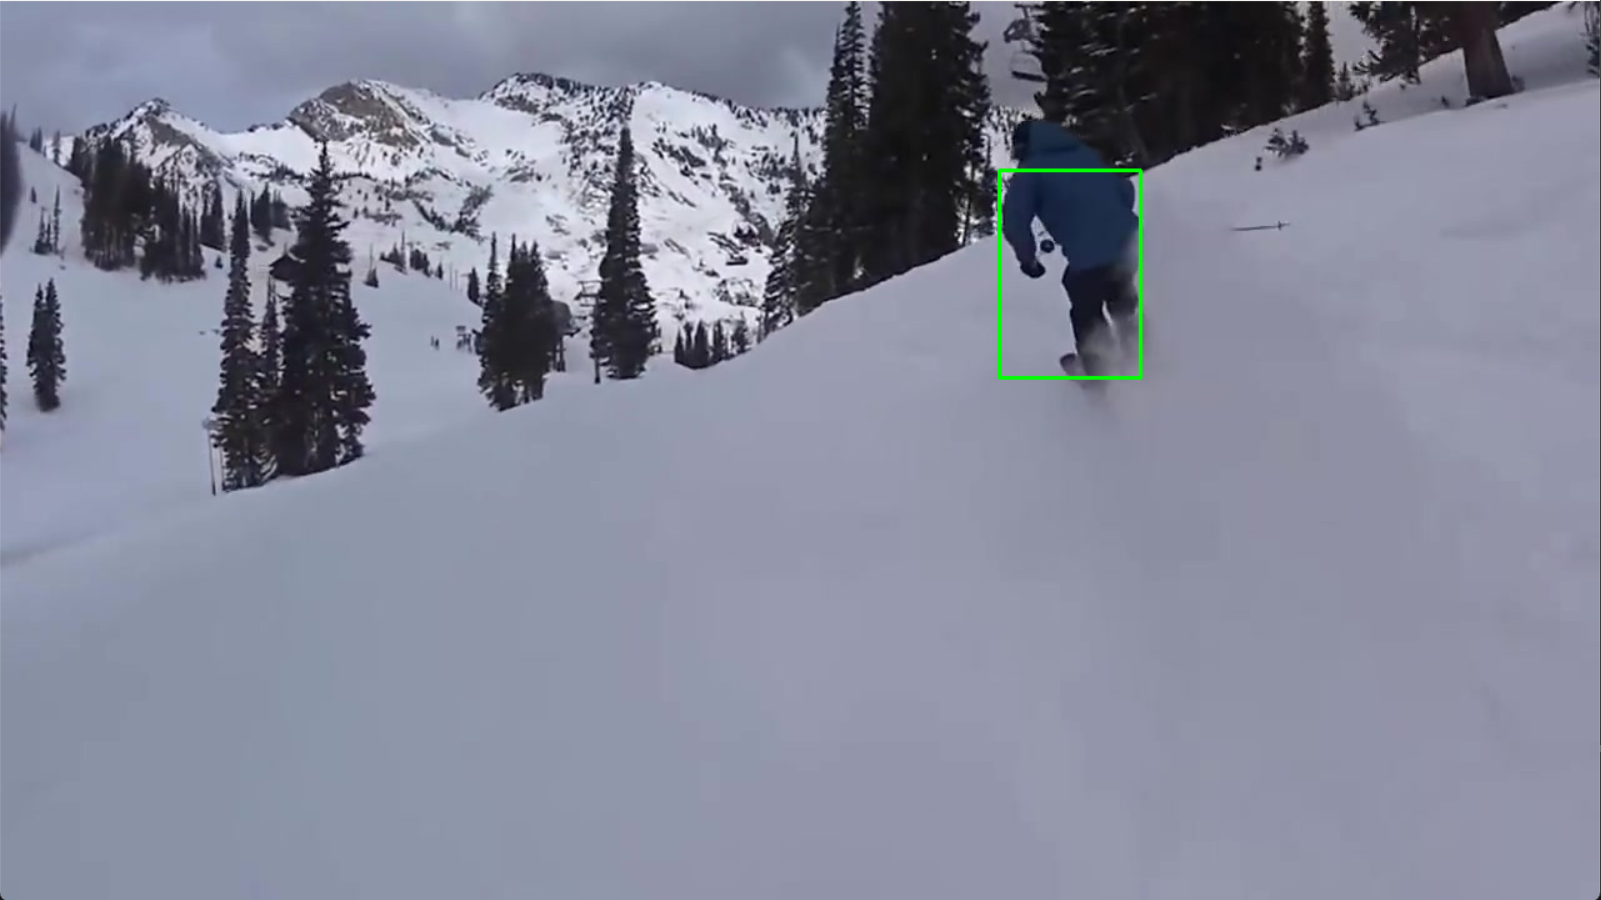
\includegraphics[width=0.48\columnwidth]{../figs/2_frame_372.png} % Row 3, Image 2
    \caption{Examples of tracker performance. In the first column we see the original tracker, it tracks the skier, then loses him when he goes off frame and then never recovers. The second column shows the modified tracker, which starts searching when it loses the target and is able to recover.}
    \label{fig:grid_3x2} % Ensure this label is unique
\end{figure}

\section{Task 6}
I implemented 2d Gaussian sampling, with the center of the Gaussian at the last known position of the target. The starting standard deviation is set to last known target size and grows to the size of the image over the course of 120 frames. The improvment can be seen on the car9 sequence, where the tracker is able to recove nearly at the same frame the car reappears. The results are shown in \ref{fig:task_6}. This method is applicable if we can assume that the target will reappear in the same are of the image. This is not always the case, such as sequence dog where there is a jump cut to a closeup of the dog leaping over an obstacle.
\begin{figure}[H]
    \centering
    \includegraphics[width=0.48\columnwidth]{../tracking_results/tracking_frame_790.jpg} \hfill
    \vspace{1ex}
    \includegraphics[width=0.48\columnwidth]{../tracking_results/tracking_frame_792.jpg} \hfill
    \vspace{1ex}
    \includegraphics[width=0.48\columnwidth]{../tracking_results/tracking_frame_794.jpg} \hfill
    \vspace{1ex}
    \includegraphics[width=0.48\columnwidth]{../tracking_results/tracking_frame_796.jpg} \hfill
    \vspace{1ex}
    \includegraphics[width=0.48\columnwidth]{../tracking_results/tracking_frame_798.jpg} \hfill
    \vspace{1ex}
    \includegraphics[width=0.48\columnwidth]{../tracking_results/tracking_frame_800.jpg} \hfill
    \vspace{1ex}
    \includegraphics[width=0.48\columnwidth]{../tracking_results/tracking_frame_802.jpg} \hfill
    \vspace{1ex}
    \includegraphics[width=0.48\columnwidth]{../tracking_results/tracking_frame_804.jpg} \hfill
    \vspace{1ex}
    \includegraphics[width=0.48\columnwidth]{../tracking_results/tracking_frame_806.jpg} \hfill
    \vspace{1ex}
    \includegraphics[width=0.48\columnwidth]{../tracking_results/tracking_frame_808.jpg} \hfill
    \vspace{1ex}
    \includegraphics[width=0.48\columnwidth]{../tracking_results/tracking_frame_810.jpg} \hfill
    \vspace{1ex}

    
    \caption{We can see the sampling growing. At the end, the tracker finds the car.}
    \label{fig:task_6} % Ensure this label is unique
\end{figure}



\section{Conclusion}
I described my work on the long-term tracking assignment. The tracker is somewhat robust to occlusions and can recover from them. The tracker is able to track the target for a long time, but it is not perfect. The tracker could be improved by making the search mode search in diffrent scales and by using a more sophisticated method to find the target. 

\bibliographystyle{IEEEtran}
\bibliography{bibliography}

\end{document}
